\section{Eigengesichter} \label{sec:eigenfaces}
\begin{tcolorbox}
	\centerline{\textbf{Lernziele Kapitel~\ref{sec:facespace}}}
	\begin{enumerate}[leftmargin=*,label=\thesection.\arabic*]
		\item \label{item:distance} Die Lernenden können den Abstand eines Punktes von einer Gerade in höheren Dimensionen berechnen.\\
		(Aufgaben~\ref{aufg:distance_simple} und~\ref{aufg:distance_complex})
		\item \label{item:eigenfaces} Die Lernenden verstehen die Konstruktion der Eigengesichter geometrisch.\\
		(Aufgaben~\ref{aufg:distance_simple} und~\ref{aufg:distance_complex})
		\item \label{item:scaling} Die Lernenden können das Minimum und das Maximum der Koeffizienten eines Vektors in Python berechnen.\\
		(Aufgabe~\ref{aufg:scaling_code})
	\end{enumerate}
\end{tcolorbox}
Die Eigengesichter werden nun aus den Differenzgesichtern konstruiert.
Wir werden zuerst nur eine bildliche Konstruktion angeben.
Dazu treffen wir folgende Annahme: Die Anzahl der Bilder $K$ sei kleiner ist als die Anzahl der Pixel $M\cdot N$ der einzelnen Bilder.
Nun stelle man sich die Differenzgesichter als eine \glqq{}Wolke\grqq{} von Punkten vor, wie rechts in Abbildung~\ref{fig:meandiff}.
\begin{enumerate}[leftmargin=2cm, label=Schritt \arabic*]
	\item Entlang einer gewissen Richtung weist diese Wolke die grösste Streuung auf.
	Entlang dieser grössten Streuung wählen wir einen Vektor $\vec u_1$ der Länge 1.
	\item \label{item:u2} Unter allen Vektoren die orthogonal zu $\vec u_1$ sind, wählen wir wieder einen, der in Richtung der grössten Streuung der Wolke zeigt.
	Diesen nennen wir $\vec u_2$ und er soll wieder Länge 1 haben.
	\item Unter allen Vektoren die orthogonal zu $\vec u_1$ und $\vec u_2$ sind, wählen wir wieder einen, der in Richtung der grössten Streuung der Wolke zeigt.
	Diesen nennen wir $\vec u_3$ und er soll wieder Länge 1 haben.
	\item Analog konstruieren wir $\vec u_4,\vec u_5,\ldots,\vec u_K$.
\end{enumerate}
Die Vektoren $\vec u_1,\ldots,\vec u_K$ heissen \textit{Eigengesichter}.
Die genaue Berechnung dieser Vektoren ist nicht so einfach und ist darum schon implementiert.
Man kann das ganze so auffassen: Mit diesem Verfahren \glqq{}lernt\grqq{} man die Eigengesichter aus der Datenbank.
Das Ganze ist links in Abbildung~\ref{fig:meandiff} stark vereinfacht visualisiert.
\begin{figure}[ht]
	\centering
	\begin{tabular}{lr}
		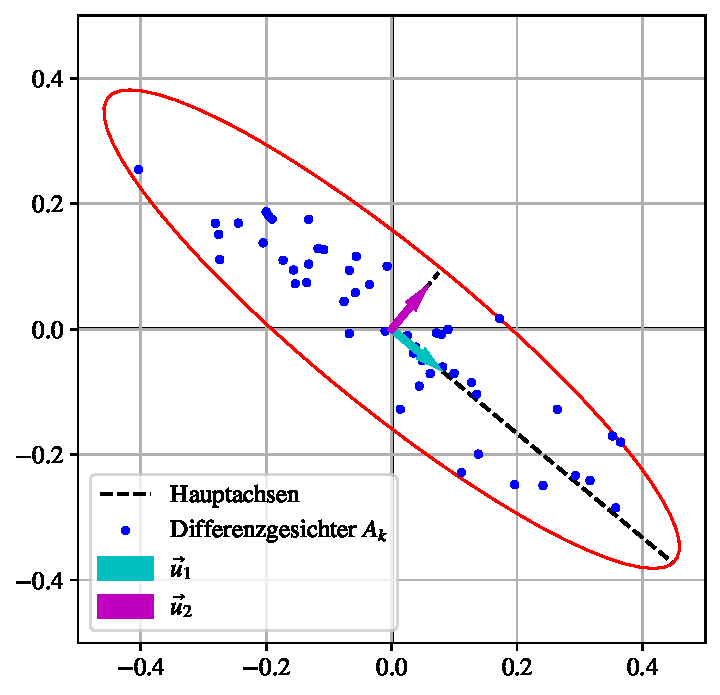
\includegraphics[width=0.45\textwidth]{images/facespace/principal_components} & 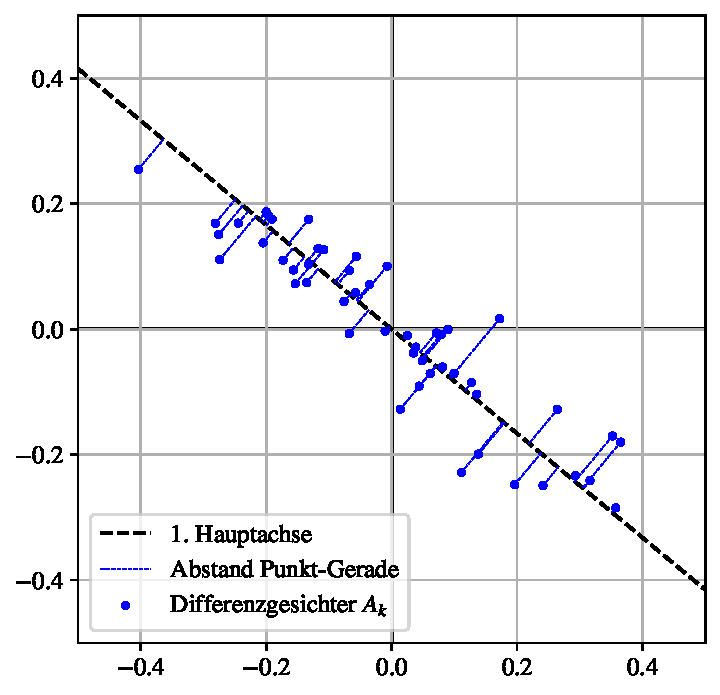
\includegraphics[width=0.45\textwidth]{images/facespace/distance_complicated} \\
	\end{tabular}
	\caption{Die Eigengesichter sind die orthonormalen Vektoren entlang den Hauptachsen.}
	\label{fig:construction}
\end{figure}

Wir werden nun das erste Eigengesicht $\vec{u}_1$ berechnen.
Dazu müssen wir zuerst verstehen was es bedeutet, einen Vektor \glqq{}entlang der grössten Streuung\grqq{} zu finden.
Die erste Hauptachse wird wie folgt bestimmt:
Sie ist diejenige Gerade, welche die Summe der Abstandsquadrate zu den $\vec{a}_1,\ldots,\vec{a}_K$ minimiert.
Dies ist rechts in Abbildung~\ref{fig:meandiff} gezeigt.
Um die Eigengesichter zu berechnen, müssen wir zuerst den Abstand eines Punktes von einer Geraden berechnen können.
\begin{aufgabe} \label{aufg:distance_simple}
	\phantom{text}\\
	\begin{minipage}{0.55\textwidth}
		Berechnen Sie den Abstand des Punktes $\vec{a}$ von der Geraden durch Null in Richtung $\vec{u}$, wobei
		\begin{align*}
			\vec{a}=
			\begin{pmatrix}
				1 \\
				-2
			\end{pmatrix},\quad
			\vec{u}=\frac{1}{5}
			\begin{pmatrix}
				4 \\
				-3
			\end{pmatrix}.
		\end{align*}
		\textit{Hinweis}: Der Vektor $\vec{u}$ hat Länge~1.
	\end{minipage}\hfill
	\begin{minipage}{0.4\textwidth}
		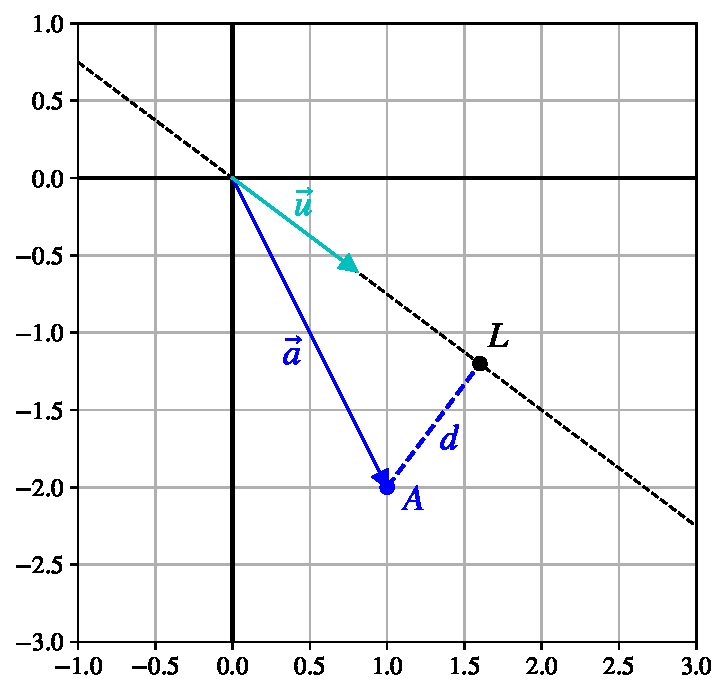
\includegraphics[width=\textwidth]{images/facespace/distance_simple}
	\end{minipage}
\end{aufgabe}
\begin{losung}
	Der Abstand des Lotfusspunktes von $\vec{a}$ zum Ursprung ist $\vec{a}\cdot\vec{u}=2$.
	Dabei haben wir verwendet, dass $\vec{u}$ Länge 1 hat.
	Die gesuchte Distanz (blaue gestrichelte Linie im Bild) bezeichnen wir mit $d$.
	Nach dem Satz von Pythagoras gilt dann
	\begin{equation*}
		d^2+\left(\vec{a}\cdot\vec{u}\right)^2=\lVert\vec{a}\rVert^2.
	\end{equation*}
	Durch umformen erhalten wir
	\begin{equation*}
		d^2=\lVert\vec{a}\rVert^2-\left(\vec{a}\cdot\vec{u}\right)^2=5-4=1.
	\end{equation*}
	Der Abstand von $\vec{a}$ zu Geraden ist also $d=1$.
\end{losung}
Was wir in Aufgabe~\ref{aufg:distance_simple} berechnet haben, funktioniert auch in höheren Dimensionen.
Seien $\vec v,\vec w\in\mathbb R^n$, wobei möglicherweise $n>3$.
Das Skalarprodukt dieser Vektoren ist dann definiert als
\begin{equation*}
	\vec v\cdot\vec w=v_1w_1+\ldots+v_nw_n.
\end{equation*}
Ganz analog ist auch das Quadrat Länge eines Vektors gegeben durch $\lVert\vec v\rVert^2=\vec v\cdot\vec v$.
Der Abstand eines Punktes zu einer Geraden berechnet sich dann nach der selben Formel wie in der Lösung von Aufgabe~\ref{aufg:distance_simple}.
\begin{aufgabe} \label{aufg:distance_complex}
	Sei $\vec{u}\in\mathbb R^{M\cdot N}$ ein Vektor der Länge~1.
	Dieser definiert die Gerade durch Null in Richtung $\vec{u}$.
	Finden Sie eine Formel für die Summe der Abstandsquadrate aller Differenzgesichter $\vec{a}_1,\ldots,\vec{a}_K$ zu dieser Geraden.
	Dies ist rechts in Abbildung~\ref{fig:construction} dargestellt.
\end{aufgabe}
\begin{losung}
	Wir konzentrieren uns zuerst auf ein beliebiges Differenzgesicht $\vec{a}_k$, wobei $k\in\left\{1,\ldots,K\right\}$.
	Dessen Abstand zur Geraden bezeichnen wir mit $d_k$.
	Analog zu Aufgabe~\ref{aufg:distance_simple} gilt
	\begin{equation*}
		d_k^2=\lVert\vec{a}_k\rVert^2-\left(\vec{a}_k\cdot\vec{u}\right)^2.
	\end{equation*}
	Die Summe dieser Abstandsquadrate $d_1^2+\ldots+d_K^2$ ist demnach gegeben durch
	\begin{equation*}
		\lVert\vec{a}_1\rVert^2-\left(\vec{a}_1\cdot\vec{u}\right)^2
		+\lVert\vec{a}_2\rVert^2-\left(\vec{a}_2\cdot\vec{u}\right)^2
		+\ldots+
		\lVert\vec{a}_{M\cdot N}\rVert^2-\left(\vec{a}_{M\cdot N}\cdot\vec{u}\right)^2.
	\end{equation*}
\end{losung}
Die Formel aus Aufgabe~\ref{aufg:distance_complex} liefert für jedes $\vec{u}$ einen positiven Wert.
Dasjenige $\vec{u}$, welches diesen Ausdruck minimiert, ist das erste Eigengesicht $\vec{u}_1$.
Die Eigengesichter zu berechnen, heisst also ein Minimierungsproblem zu lösen.
Dies ist nicht so einfach und ist daher bereits implementiert.

Die Eigengesichter wollen wir nun visualisieren, indem wir sie wieder als Bilder darstellen.
Doch da gibt es noch ein Problem.
Die Komponenten der Eigengesichter liegen nicht notwendigerweise in $\left[0,1\right]$.
Damit man sie als Bilder darstellen kann, müssen wir deren Komponenten zuerst auf geeignete Weise nach $\left[0,1\right]$ abbilden.
Das geht wie folgt:
Sei $\vec v\in\mathbb R^{M\cdot N}$ irgend ein Vektor, dessen Komponenten nicht notwendigerweise in $\left[0,1\right]$ liegen.
Sei $\min\left(\vec v\right)$ das Minimum und $\max\left(\vec v\right)$ das Maximum aller Komponenten von $\vec v$.
Wir betrachten nun den Vektor
\begin{equation*}
	\vec w=
	\begin{pmatrix}
		w_1 \\
		w_2 \\
		\vdots \\
		w_{M\cdot N}
	\end{pmatrix}
\end{equation*}
dessen Komponenten sich aus denen von $\vec v$ wie folgt zusammensetzen
\begin{equation*}
	w_i=\frac{v_i-\min\left(\vec v\right)}{\max\left(\vec v\right)-\min\left(\vec v\right)},
\end{equation*}
für alle $i\in\left\{1,\ldots,M\cdot N\right\}$.
Die Komponenten des Vektors $\vec w$ liegen dann alle in $\left[0,1\right]$.
Falls alle Komponenten von $\vec v$ gleich sind, ist $\min\left(\vec v\right)=\max\left(\vec v\right)$ und wir haben eine Division durch Null.
Wir ignorieren diesen Fall.
\begin{aufgabe} \label{aufg:scaling_theory}
	\phantom{text}
	\begin{enumerate}[label=(\alph*)]
		\item Betrachten Sie den Vektor
		\begin{equation*}
			\vec v=
			\begin{pmatrix}
				-2 \\
				4 \\
				1
			\end{pmatrix},
		\end{equation*}
		dessen Komponenten nicht alle in $\left[0,1\right]$ liegen.
		Berechnen Sie daraus den Vektor $\vec w$ gemäss obigem Verfahren.
		\item Begründen Sie, warum dieses Verfahren immer einen Vektor mit Komponenten in $\left[0,1\right]$ liefert, auch für einen allgemeinen Vektor $\vec v$ (dessen Komponenten nicht alle gleich sind).
	\end{enumerate}
\end{aufgabe}
\begin{losung}
	\phantom{text}
	\begin{enumerate}[label=(\alph*)]
		\item In obigem Beispiel ist $\min\left(\vec v\right)=-2$ und $\max\left(\vec v\right)=4$.
		Daraus ergibt sich für alle $i\in\left\{1,2,3\right\}$
		\begin{equation*}
			w_i=\frac{v_i-\left(-2\right)}{4-\left(-2\right)}=\frac{v_i+2}{6}.
		\end{equation*}
		Somit erhalten wir
		\begin{equation*}
			\vec w=
			\begin{pmatrix}
				0 \\
				1 \\
				\tfrac{1}{2}
			\end{pmatrix}.
		\end{equation*}
		\item Für alle Komponenten $v_i$ gilt stets
		\begin{equation*}
			\min\left(\vec v\right)\leq v_i\leq\max\left(\vec v\right).
		\end{equation*}
		Daraus folgt, dass im Bruch
		\begin{equation*}
			w_i=\frac{v_i-\min\left(\vec v\right)}{\max\left(\vec v\right)-\min\left(\vec v\right)},
		\end{equation*}
		der Nenner immer grösser oder Gleich dem Zähler ist, und dass beide nicht negativ werden können.
		Folglich muss $w_i\in\left[0,1\right]$ gelten.
	\end{enumerate}
\end{losung}
\begin{aufgabe} \label{aufg:scaling_code}
	Ergänzen Sie die Funktion \texttt{interpolate(v)}, welche den Vektor mit Komponenten in $\left[0,1\right]$ zurück gibt, der aus dem Vektor \texttt{v} durch obiges Verfahren entsteht.
	Testen Sie ihre Lösung mit dem Python Skript \texttt{plot\_eigenfaces.py}, welches ihre Funktion \texttt{interpolate(v)} auf die Eigengesichter $\vec u_1,\ldots,\vec u_K$ anwendet und diese als Bilder abspeichert.
	\textit{Hinweis:} Die Funktionen \texttt{np.min(v)} und \texttt{np.max(v)} liefern das Minimum und das Maximum eines Vektors \texttt{v}.
\end{aufgabe}
\begin{losung}
	Eine mögliche Lösung ist unten gezeigt.
	Die Eigengesichter sind in Abbildung~\ref{fig:eigenfaces} dargestellt.
	\begin{lstlisting}[style=python]
		import numpy as np
		
		def interpolate(v):
		w = np.zeros_like(v)
		a = np.min(v)
		b = np.max(v)
		for vi, wi in zip(v, w):
		wi = (vi - a) / (b - a)
		return w
	\end{lstlisting}
\end{losung}

\begin{figure}[ht]
	\centering
	\begin{tabular}{cccccccc}
		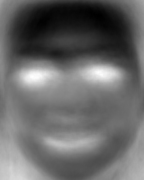
\includegraphics[width=0.1\textwidth]{images/eigenfaces/eigenface00} & 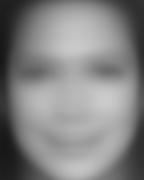
\includegraphics[width=0.1\textwidth]{images/eigenfaces/eigenface01} &
		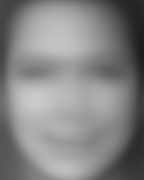
\includegraphics[width=0.1\textwidth]{images/eigenfaces/eigenface02} & 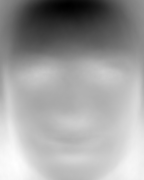
\includegraphics[width=0.1\textwidth]{images/eigenfaces/eigenface03} &
		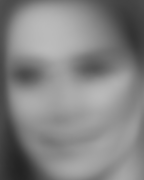
\includegraphics[width=0.1\textwidth]{images/eigenfaces/eigenface04} &
		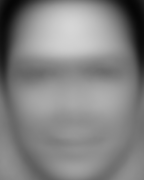
\includegraphics[width=0.1\textwidth]{images/eigenfaces/eigenface05} & 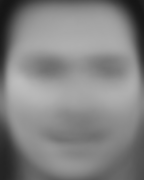
\includegraphics[width=0.1\textwidth]{images/eigenfaces/eigenface06} &
		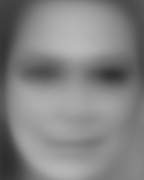
\includegraphics[width=0.1\textwidth]{images/eigenfaces/eigenface07} \\ 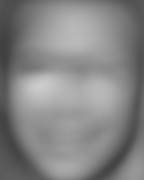
\includegraphics[width=0.1\textwidth]{images/eigenfaces/eigenface08} &
		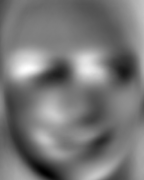
\includegraphics[width=0.1\textwidth]{images/eigenfaces/eigenface09} & 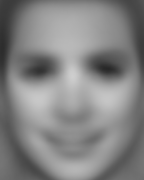
\includegraphics[width=0.1\textwidth]{images/eigenfaces/eigenface10} &
		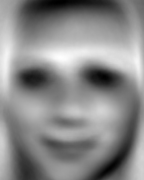
\includegraphics[width=0.1\textwidth]{images/eigenfaces/eigenface11} & 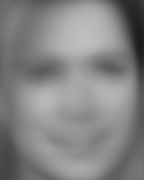
\includegraphics[width=0.1\textwidth]{images/eigenfaces/eigenface12} &
		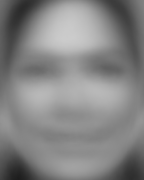
\includegraphics[width=0.1\textwidth]{images/eigenfaces/eigenface13} & 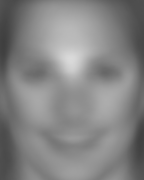
\includegraphics[width=0.1\textwidth]{images/eigenfaces/eigenface14} &
		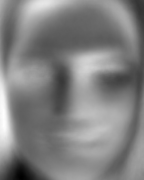
\includegraphics[width=0.1\textwidth]{images/eigenfaces/eigenface15} \\
	\end{tabular}
	\caption{Die ersten 16 Eigengesichter wurden wieder als Bild dargestellt.}
	\label{fig:eigenfaces}
\end{figure}

Im Grunde fangen die Eigengesichter charakteristische Gesichtszüge ein.
Mit charakteristisch ist hier gemeint, dass genau diese Gesichtszüge für die grösste Streuung unter allen Bildern der Datenbank verantwortlich sind.
Sie beschreiben die Merkmale, nach denen sich die Gesichter am meisten unterscheiden.
Besser gesagt: Das erste Eigengesicht fängt den Gesichtszug mit der grössten Streuung ein.
Die weiteren Eigengesichter fangen Gesichtszüge mit immer weniger Streuung ein.
Dies spiegelt sich auch in deren Konstruktion wieder, welche die Eigengesichter ja gerade als Vektoren entlang der grössten Streuung definiert.